\vspace{-1.5cm}
\small
\textbf{The results in this chapter are published as:}
\vspace{0.05 cm}

% We cite the paper with fontsize 10
\fullcite{Abella-2022-AME}
\normalsize
\vspace{0.5 cm}

In this chapter, we analyze the aging implications in one of the simplest binary-state threshold models: the Granovetter-Watts model. Our analytical approximations give a good description of extensive Monte Carlo simulations in Erd\H{o}s-R\'enyi, random-regular and Barab\'asi-Albert networks. While aging does not modify the cascade condition, it slows down the cascade dynamics towards the full-adoption state: the exponential increase of adopters in time from the original model is replaced by a stretched exponential or power law, depending on the aging mechanism. Under several approximations, we give analytical expressions for the cascade condition and for the exponents of the adopters' density growth laws. Beyond random networks, we also describe by Monte Carlo simulations the effects of aging for the Granovetter-Watts model in a two-dimensional lattice.

\section{\label{sec:Introduction_Threshold} Introduction}

The Granovetter-Watts model~\cite{granovetter-1978,watts-2002}, is a well-known binary-state model for Complex contagion processes, such as rumor propagation,  riots, stock market herds, adoption of new technologies, political and environmental campaigns, etc. The discontinuous phase transition and the cascade condition exhibited by the Granovetter-Watts model were predicted with analytical tools in Ref.~\cite{watts-2002}. This model has been extensively studied in regular lattices and small-world networks~\cite{centola-2007}, random graphs~\cite{gleeson-2007},  modular and community structure~\cite{gleeson-2008}, clustered networks~\cite{hackett-2011,hackett-2013}, hypergraphs~\cite{de-arruda-2020}, homophilic networks~\cite{diaz-diaz-2022}, etc. Moreover, recent studies also include variants of the adoption rules including
%social reinforcement in multiple layers~\cite{chen-2018}, 
the impact of opinion leaders~\cite{liu-2018} and seed-size~\cite{singh-2013}, on-off threshold~\cite{dodds-2013} and the competition between simple and complex contagion~\cite{czaplicka-2016,min-2018,min-2018-dual,diaz-diaz-2022,min2023threshold}. Additionally, the Granovetter-Watts model has been confronted with several sources of empirical data~\cite{centola-2010,karimi-2013,karsai-2014,rosenthal-2015,karsai-2016,mnsted-2017,unicomb-2018,guilbeault-2021}.


Previous studies of the Granovetter-Watts model usually rely on a Markovian assumption for the dynamics. This implies that events depend only on the present state, i.e., dynamical rules are memoryless. Markovian processes exhibit exponential distributions in the upcoming event times and the number of events in a given time interval follows a Poisson distribution. However, there is strong empirical evidence against this assumption in human interactions and thus, the understanding of these non-Markovian effects is in general a topic of current interest~\cite{van-mieghem-2013,starnini-2017,peralta-2020C,peralta-2020A}. In particular, for the threshold models, memory effects have been included as past exposures' memory~\cite{dodds-2004}, message-passing algorithms~\cite{shrestha-2014}, memory distributions for retweeting algorithms~\cite{gleeson-2016} and timers~\cite{oh-2018}.

Regarding the specific context of innovation adoption from the complex systems point of view~\cite{przybyla2014diffusion}, mechanisms of inertia or resistance to adopt the technology have been already introduced. In fact, the original approach of Rogers~\cite{rogers2014} considers a fraction of ``laggards'' that will resist innovating until a large majority of the population has already adopted it. Other works highlight the importance of timing interactions~\cite{bass1969} and the effect of ``contrarians'' (tendency to act against the majority), which has an important impact on the dynamics~\cite{galam-2008,goncalves-2012}. In Ref.~\cite{goncalves-2012}, it is discussed how different technologies may show different adoption cascades regarding the balance between advertisement and resistance to change.

In this chapter, we incorporate the aging mechanism into the Granovetter-Watts model, characterizing both the cascade condition and dynamics towards the fully adopted state. We propose two different aging mechanisms giving rise to heterogeneous activity patterns, characterized by flat-tail inter-event time distributions. To describe the results, we use the general master equation for any binary-state model with temporal activity patterns previously described in Chapter \ref{ch:Aging in binary state dynamics}. For the particular case of the Granovetter-Watts model, we are able to reduce the dimensionality of the full system without loss of accuracy. Theoretical predictions are matched with extensive Monte Carlo simulations in different networks. For completeness, the role of both aging mechanisms is also studied in a two-dimensional Moore lattice.

The chapter is organized as follows. In the next section, we describe the original Granovetter-Watts model and introduce exogenous and endogenous aging in the model. In Section \ref{sec:Complex networks}, numerical results are reported and contrasted with theoretical predictions for different complex networks. For completeness, in Section \ref{sec:Lattice} the case of a 2D-lattice is analyzed. The final section contains a summary and a discussion of the results.

\begin{figure}
    \centering \captionsetup{font=sf}
    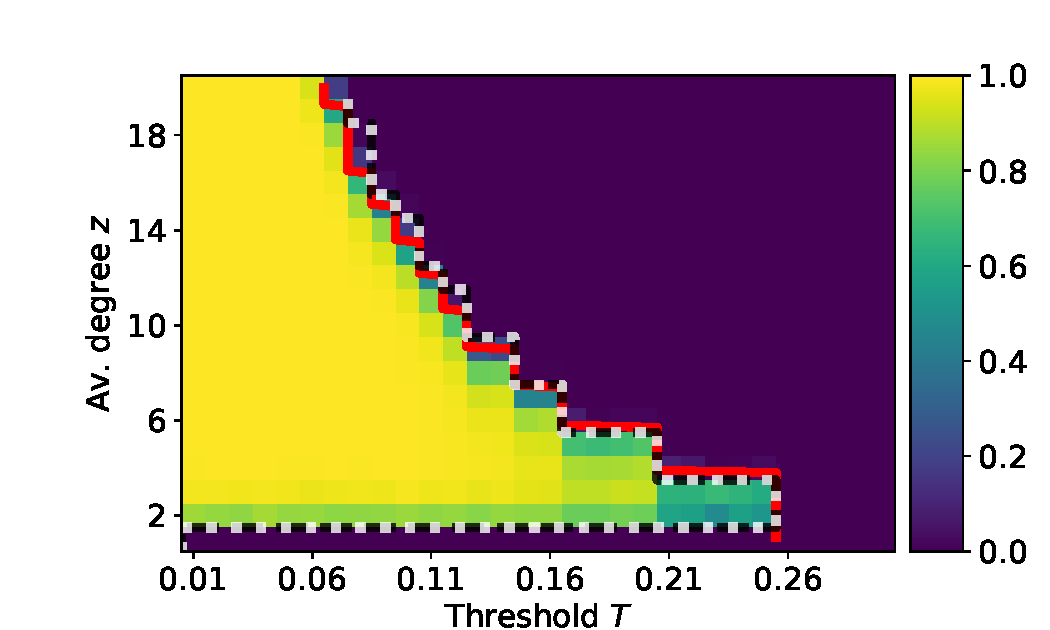
\includegraphics[width=0.65\columnwidth]{Figs/Aging_Threshold/cascade.pdf}
    \caption[Average density $x^{-}$ of adopters for an Erd\H{o}s-R\'enyi graph]{\label{fig:umbral} Average density $x^{-}$ of adopters for an Erd\H{o}s-R\'enyi graph of mean degree $z$ using a model with threshold $T$. Color-coded values of $x^{-}$ are from Monte Carlo simulations of the model without aging in a graph with $N = 10,000$ agents.  Black dashed and white dotted lines correspond to $T_c$ value obtained numerically for the model with exogenous and endogenous aging, respectively.  Monte Carlo simulations are averaged over $M = 5 \times 10^4$ realizations. The red solid line is the analytical approximation of the cascade boundary, from Eq. \eqref{eq:linear}, which is the same with and without aging.}
\end{figure}

\section{\label{sec:Threshold model with aging} Aging in the Granovetter-Watts model}

As it was introduced before (see Section \ref{sec:Granovetter-Watts threshold model}), the standard Granovetter-Watts model~\cite{granovetter-1978,watts-2002} considers a network of $N$ interacting agents, where each node of the network represents an agent $i$ with a binary-state variable $\sigma_i = \left\{ 0,1 \right\}$  and a given threshold $T$ ($0<T<1$). The state indicates if the agent has adopted a technology (or joined a riot, spread a meme or fake news, etc.) or not. We use the wording of a technology adoption process for the rest of the chapter. If a node $i$ (with $k$ neighbors) has not adopted  ($\sigma_i = 0$) the technology, becomes adopter ($\sigma_i = 1$) if the fraction $m / k$ of neighbors adopters exceeds the threshold $T$. Adopter nodes cannot go back to the non-adopter state.

In the Granovetter-Watts model with aging, each agent has an internal time $j = 0,1,2,...$  (in Monte-Carlo units) as in Refs.~\cite{fernandez-gracia-2013,artime-2018,peralta-2020C,peralta-2020A,chen-2020,fernandez-gracia-2011,perez-2016,stark-2008}.  As initial condition, we set $j = 0$ for all nodes. In Monte Carlo simulations, we follow a Random Asynchronous Update in which agents are activated in discrete time steps with probability $p_{A} (j) = 1/(j+2)$. When a non-adopter agent is activated, she changes state according to the threshold condition $m/k > T$. We will consider two different aging mechanisms, endogenous and exogenous aging~\cite{fernandez-gracia-2011}, which account for the power law inter-event time distributions empirically observed in human interactions~\cite{artime-2017}. For endogenous aging,  the internal time measures the time spent in the current state: If an agent in an updating attempt is not activated or does not adopt, the internal time increases by one unit. Therefore, the longer an agent has remained without adopting the technology, the more difficult it is for her to adopt it. 

For exogenous aging, the internal time accounts for the time since the last attempt to change state: In each updating attempt in which the agent is activated, the internal clock resets to $j = 0$ even if there is no adoption. In this case, aging is understood as a resistance to adopt the technology the longer the agent has not been induced to consider adoption by some external influence.  

%In this chapter, we explore the effects of another aging mechanism: the exogenous aging~\cite{fernandez-gracia-2013}. In this case, we consider failed adoption attempts as separate events in which the persistence time is reset. In other words, if an agent activates and does not change state (the case when $m/k \leq T$), the internal time is also reset to $j = 0$. Therefore, the internal time $j$ accounts for the time spent in the current state or since the last attempt to change state. This mechanism is introduced to model the propensity of some agents to change by some external influence (social media, political situation...) even if they are surrounded by an unfavorable environment. In addition, this type of aging allows us to explore how temporal heterogeneities affect the cascade dynamics.

\begin{figure}
    \centering \captionsetup{font=sf}
    \includegraphics[width=0.55\columnwidth]{Figs/Aging_Threshold/GRAPH_PLOT.pdf}
    \caption[Cascade spreading for the Granovetter-Watts model]{\label{fig:graph_plot} Cascade spreading for the original Granovetter-Watts model \textbf{(a)}, and the versions with endogenous (reset if adopts) \textbf{(b)} and exogenous (reset if activates) \textbf{(c)} aging. Yellow nodes are adopters and purple nodes are non-adopters. Time increases from left to right. Monte Carlo simulations are performed in an Erd\H{o}s-R\'enyi network with mean degree $z = 3$ and $T = 0.22$. System size is $N = 8,000$.}
\end{figure}

\section{\label{sec:Complex networks} Results  on Complex networks}

In this section we discuss the Granovetter-Watts model with endogenous and exogenous aging in three different complex networks: random-regular (RR)~\cite{wormald_1999}, Erd\H{o}s-R\'enyi (ER)~\cite{erdos1960evolution} and Barab\'asi-Albert (BA)~\cite{barabasi2009scale}.

\subsection{\label{subsec:Numerical results} Numerical results}

For the networks considered, the Granovetter-Watts model undergoes a discontinuous phase transition at a certain critical value $T_{c}$ (cascade condition)~\cite{watts-2002}. For $T<T_c$, a small initial seed of adopters triggers a global cascade where, on average, a significant proportion of agents in the system adopt the technology (change from $\sigma_i = 0 \mbox{ to } \; 1$). In our analysis, the initial condition is set to favor cascades: one agent $i$ with degree $k_i = z$ is selected randomly and all her neighbors are initially adopters, as in Ref.~\cite{centola-2007,singh-2013}. For $T>T_c$, there are few cascade occurrences and none of them is global. The cascade condition dependence with the average degree $z$ of the underlying network has been studied in Refs.~\cite{watts-2002, gleeson-2007}. For the two aging mechanisms considered, Monte Carlo simulations in random graphs show that the $T_c$ dependence on $z$ is very similar to the one for the model without aging (see Fig. \ref{fig:umbral}). Therefore, for random networks, tends to the same cascade condition derived for the original model (which for ER graphs is $T_{c} = 1 / z$~\cite{watts-2002}). Similar results were found for RR and BA graphs. This result is not obvious a priory because aging has been shown to modify the final state in several models~\cite{fernandez-gracia-2013,artime-2018,peralta-2020C,peralta-2020A,chen-2020,fernandez-gracia-2011,perez-2016,stark-2008}. 

Even though aging in the Granovetter-Watts model does not modify the cascade condition, it has a large impact in the complex contagion cascade dynamics (Fig.\ref{fig:graph_plot}). 
%In Refs.~\cite{gleeson-2008,gleeson-2013}, the authors described the fraction of adopted agents $x^{-}(t)$ evolution as a solution of a master equation. 
From Monte Carlo simulations in a random regular graph we find that, without aging,  the average fraction of adopters, denoted by $x^{-}$, follows an initial exponential increase with time (see Fig. \ref{fig:graph_plot}a and \ref{fig:models}a), 
\begin{equation}
x^{-}(t) \sim x^{-}_{0} \, e^{\alpha \, t},
\label{eq:exponential}
\end{equation}
where $x^{-}_{0}$ is the initial fraction of adopters (seed). This behavior is universal for all values of the control parameters $z$ and $T$ below the cascade condition. In addition, we investigated the approach to the full-adopt state ($x^{-} = 1$) and we found that the fraction of non-adopters, denoted by $x^{+}$, follows an exponential decay for all values of the control parameters (see inset in Fig.\ref{fig:models}a).

\begin{figure}
\centering \captionsetup{font=sf}
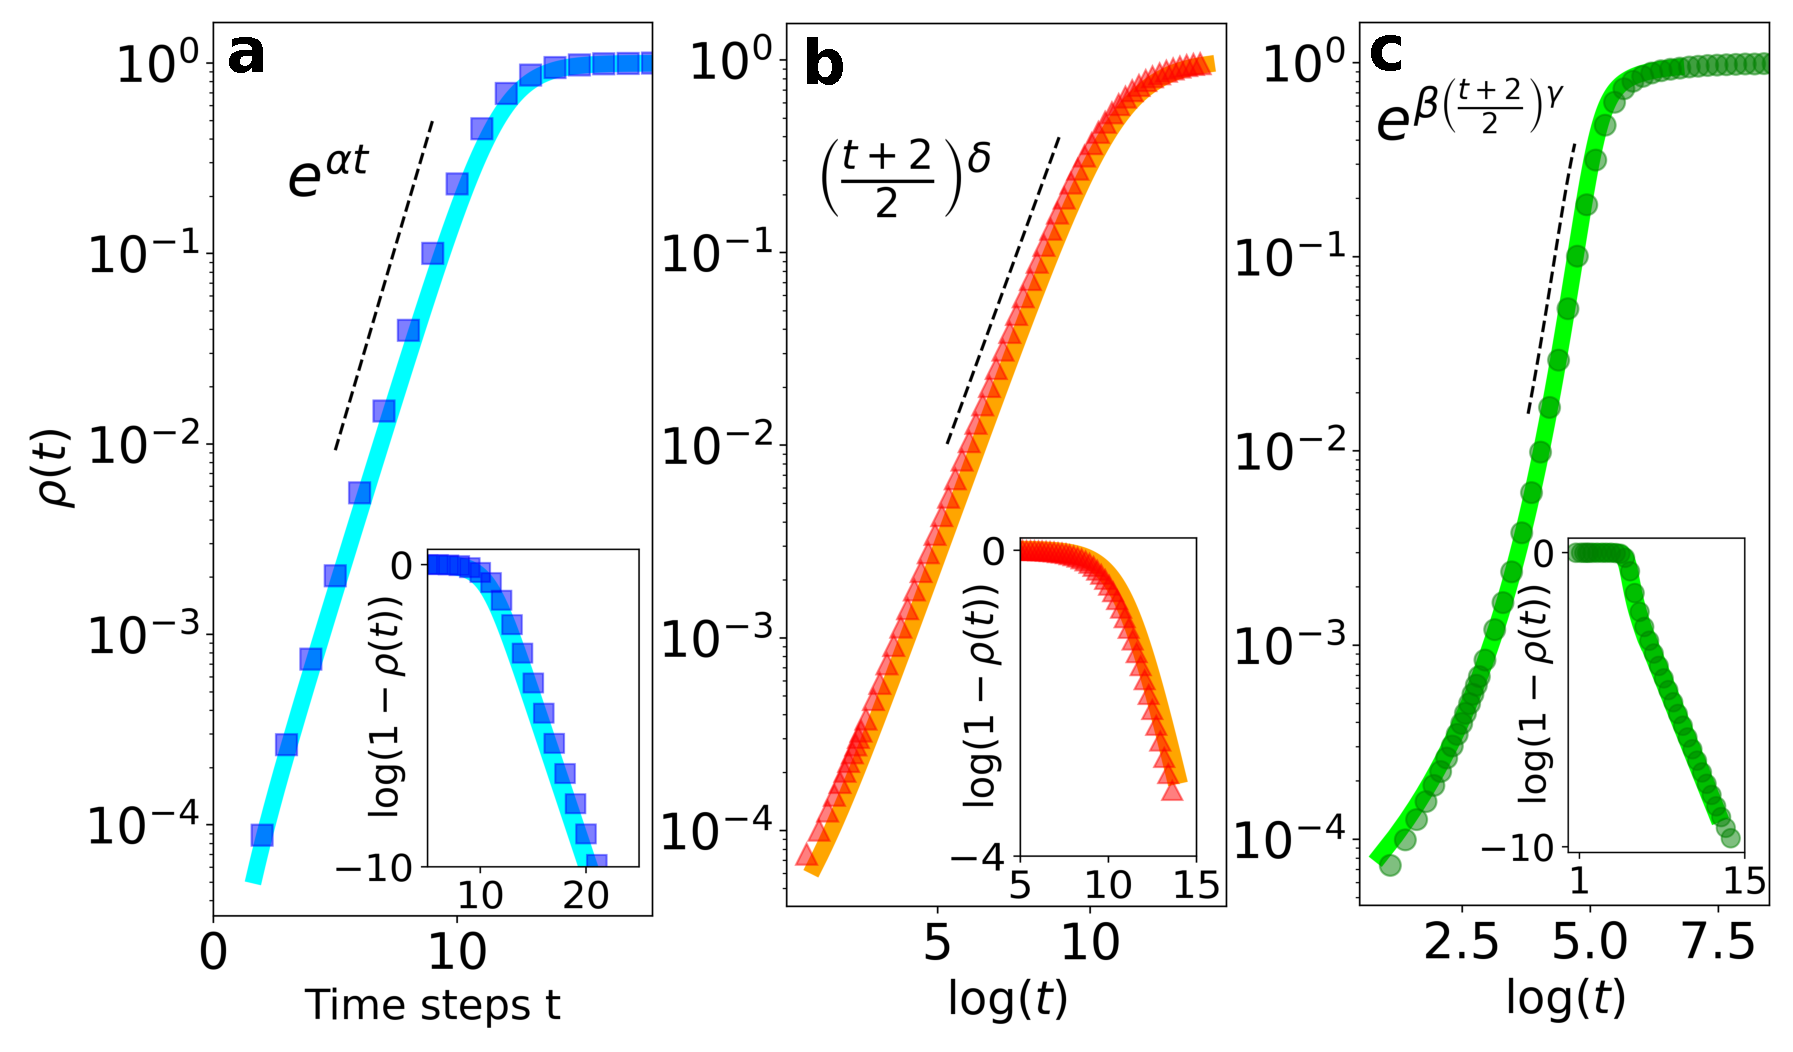
\includegraphics[width=0.8\columnwidth]{Figs/Aging_Threshold/EVO_MOD.pdf}
\caption[Cascade dynamics and fall to the full-adopt state ($x^{-} \sim 1$)]{\label{fig:models} Cascade dynamics and fall to the full-adopt state ($x^{-} \sim 1$) of the Granovetter-Watts model without aging \textbf{(a)} and the versions with endogenous \textbf{(b)} and exogenous \textbf{(c)} aging effects. At (b-c), the evolution is plotted as a function of the logarithm of time $\log{(t)}$ in Monte Carlo steps, as in the insets. The underlying network is a 3-regular random graph and the threshold is $T = 0.2$. The exponent values are $\alpha \simeq 1.0$, $\beta \simeq 1.14$, $\gamma \simeq 0.38$ and $\delta \simeq 1.0$. Numerically integrated solutions of Eq. \eqref{eq:AME_Threshold} (solid lines) describe accurately the numerical results. Monte Carlo simulations are averaged over $M = 5 \times 10^4$ realizations in a network of $N = 1.6 \times 10^5$ nodes.}
\end{figure}

When aging is introduced, the cascade dynamics are much slower than an exponential law (see Fig. \ref{fig:graph_plot}b). For endogenous aging, all non-adopters agents have the same activation probability $p_A(j)$, which decreases at each time step. This gives rise to cascade dynamics well-fitted by a power law increase (see Fig. \ref{fig:models}b),
\begin{equation}
x^{-}(t) \sim x^{-}_0 \, \left( \frac{t + 2}{2}\right)^\delta .
\label{eq:power law}
\end{equation}
For exogenous aging, we observe a slow adoption spread at the beginning followed by a cascade where almost all agents adopt the technology (Fig. \ref{fig:graph_plot}c). This behavior is well-fitted with a stretched exponential increase of the number of adopters (see Fig. \ref{fig:models}c),
\begin{equation}
x^{-}(t) \sim  x^{-}_0\,  e^{\beta \, ((t + 2) / 2)^{\gamma}} .
\label{eq:streched_exp}
\end{equation}
For both aging mechanisms, in the last stages of evolution, a few ``stubborn'' non-adopters remain, although the environment favors the adoption. Due to the chosen activation probability, the number of non-adopters decay with a power law $x^{+}(t) \sim 1/(t+2)$ in both cases (see insets at Fig. \ref{fig:models}(b-c)).

\begin{figure}
\centering \captionsetup{font=sf}
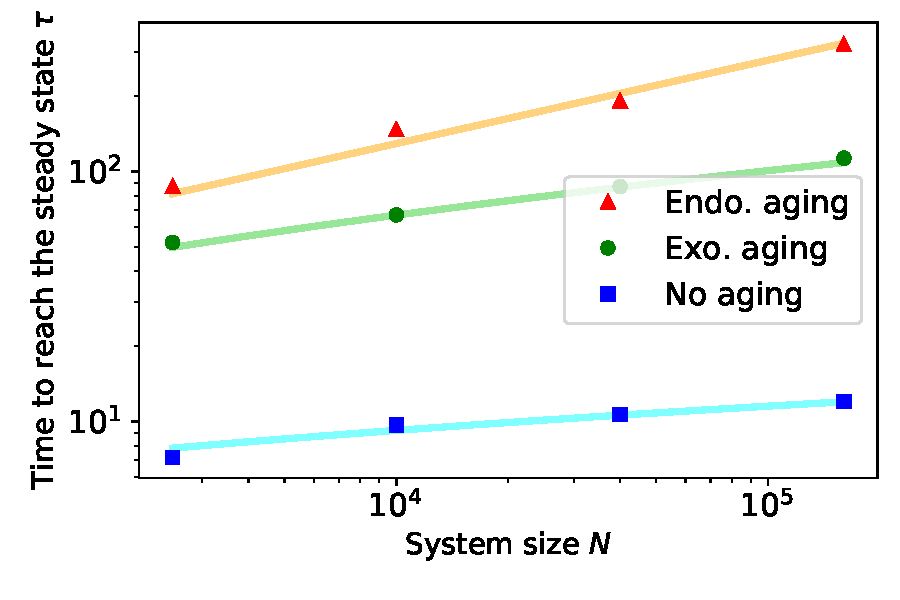
\includegraphics[width=0.6\columnwidth]{Figs/Aging_Threshold/time_steady.pdf}
\caption[Average time to reach the steady state $\tau$]{\label{fig:time_steady} Average time to reach the steady state ($x^{-} > 0.9$) $\tau$ as a function of the system size $N$ for the original Granovetter-Watts model and the versions with endogenous and exogenous aging. The underlying network is a 5-regular random graph and the threshold is $T = 0.12$. Monte Carlo simulations are averaged over $M = 5 \times 10^4$ realizations. Solid lines are the system size-dependent timescale: For the original model, $\tau_{\rm{NO AG.}} = (1/\alpha)\log(N)$, for the endogenous $(\tau_{\rm{ENDO}} = 2N^{1/\delta} - 2)$ and for the exogenous aging ($\tau_{\rm{EXO}} = 2(\log(N)/\beta)^{1/\gamma} - 2$), which follows from the dynamics from Eq. \eqref{eq:exponential}, \eqref{eq:power law} and \eqref{eq:streched_exp}. The exponents $\alpha$, $\beta$, $\gamma$ and $\delta$ are fitted exponents from numerical simulations.}
\end{figure}

Comparing the evolution of the original model with one of the versions with aging, we observe an important separation of time scales. While for the original model, the time to reach the steady state follows a logarithmic increase with the system size, the versions with endogenous and exogenous aging show a power law and a power-logarithmic dependence, respectively (see Fig.\ref{fig:time_steady}). Therefore, the time scale separation between the original model and the versions with aging increases as we increase the system size, and thus, the aging effects are more relevant for large systems.

The power law and the stretched exponential dynamics for endogenous and exogenous aging, respectively, are observed for $z$ and $T$ below the cascade condition ($T < T_c$) and for many different system sizes. This is shown in Fig. \ref{fig:exo_endo_evo} for a random regular, Erd\H{o}s-R\'enyi and  Barab\'asi-Albert networks. In particular, we show that the time-dependent behavior for different system sizes collapses to a single curve when time is scaled with the system size-dependent timescale (previously analyzed in Fig. \ref{fig:time_steady}) that follows from either the power law dynamics $(\tau_{\rm{ENDO}} = 2N^{1/\delta} - 2)$  or the stretched exponential law  $(\tau_{\rm{EXO}} = 2( \log(N)/\beta )^{1/\gamma} - 2)$. Notice that the scaling of the y-axis is necessary for Fig.\ref{fig:exo_endo_evo}(d-f) to show a linear dependence due to the stretched exponential increase.

%d for the different system sizes considering the numerically fitted dependence: stretched exponential for exogenous aging and power law for the endogenous case. Thus, these cascade dynamics are universal for any system size. The variation of parameters $z$ and $T$ only change the exponent values: $\gamma(z,T)$ and $\delta(z,T)$. The exponent dependence is different for graphs with different degree distribution $p_k$. Fig.\ref{fig:exo_endo_evo} shows the particular case for the 3 networks chosen. In particular, for a random-regular graph, the exponents do not depend on the parameter $T$ ($\gamma(z)$ and $\delta(z)$). For the other graphs considered, approaching $T$ to $T_c$ slows cascade dynamics in both cases ($\gamma(z,T)$ and $\delta(z,T)$ decrease). 

A different question is the dependence of the exponents of the power law and stretched exponential with the parameters $z$ and $T$. Numerical results from fitted Monte Carlo simulations for $\alpha(z,T)$, $\delta(z,T)$ and $\gamma(z,T)$ are shown in Figs. \ref{fig:endo_exp} and \ref{fig:exo_exp}. For a random-regular graph, as apparent from Fig. \ref{fig:exo_endo_evo}, the exponents do not depend on the parameter $T$ up to $T_c$ (so the exponents are dependent only on $z$, $\alpha(z)$, $\gamma(z)$ and $\delta(z)$), while for Erd\H{o}s-R\'enyi and Barab\'asi-Albert networks the value of the exponents decrease with $T$ when approaching $T_c$, indicating a slowing down of the dynamics. Also, for these two latter networks, the exponents present a maximum value at a certain value of $z$. This maximum value at a certain $z$ for a fixed $T$ can be understood as being between the two critical lines of Fig. \ref{fig:umbral}.

\subsection{\label{subsec:Approximate master equation and solutions} General mathematical description}

\begin{figure}[t]
    \centering \captionsetup{font=sf}
    \includegraphics[width=\linewidth]{Figs/Aging_Threshold/FIG_EVO_EXO_ENDO.pdf}
    \caption[Cascade dynamics of the Granovetter-Watts model in graphs]{\label{fig:exo_endo_evo} Cascade dynamics of the Granovetter-Watts model with endogenous (a - c) and exogenous (d - f) aging. From the left column to the right: a random regular graph with degree $z=5$ (a and d), an Erd\H{o}s-R\'enyi graph with average degree $z = 5$ (b and e) and a Barab\'asi-Albert graph with average degree $z = 8$ (c and f). Different colors indicate different values of $T$ and markers correspond to different system sizes: $N = 2,500$ (plus), $10,000$ (circles), $40,000$ (triangles), $160,000$ (crosses) and $640,000$ (squares). Time is scaled according to the system size for each model: $\tau_{\rm{EXO}} = 2(\log(N)/\beta)^{1/\gamma} - 2$, $\tau_{\rm{ENDO}} = 2N^{1/\delta} - 2$, where $\beta$,$\gamma$ and $\delta$ are the fitted exponents from the behavior according to Eq. \eqref{eq:power law} and \eqref{eq:streched_exp}. Solid lines are obtained from the solutions of Eq. \eqref{eq:PA}. Monte Carlo simulations are averaged over $M = 5 \times 10^4$ realizations.}
\end{figure}

To account for the non-Markovian dynamics introduced by the aging mechanism, we need to go beyond the standard mathematical descriptions of the Granovetter-Watts model~\cite{gleeson-2007,gleeson-2008,gleeson-2013}. We do so using a Markovian description by enlarging the number of variables~\cite{peralta-2020C,peralta-2020A}. Namely, we classify the agents with degree $k$, number of adopter neighbors $m$ and age $j$ as different sets in a compartmental model in a general framework for binary-state dynamics in complex networks, as described in Chapter \ref{ch:Aging in binary state dynamics}. To write down the AME for the Granovetter-Watts model with aging, we need to consider the following possible transitions:
\begin{itemize}
    \item A node $i$, in state $\sigma_i = \pm 1$, changes state and resets internal age with probability $T^{\pm} (k,m,j)$;
    \item A node $i$, in state $\sigma_i = \pm 1$, remains in the same state and resets internal age to zero ($j \to 0$) with probability $R^{\pm} (k,m,j)$;
    \item A node $i$, in state $\sigma_i = \pm 1$, remains in the same state and ages ($j \to j+1$) with probability $A^{\pm} (k,m,j)$.
\end{itemize}
For the specific case of the Granovetter-Watts model, dynamics are monotonic and $T^{-} (k,m,j) = 0$ (no adopter becomes a non-adopter). Moreover, when an agent becomes an adopter, there are neither resetting nor aging events $R^{-} (k,m,j) = A^{-} (k,m,j) = 0$. This means as well that equations for the non-adopters $x^{+}_{k,m,j}$ and adopters $x^{-}_{k,m,j}$ nodes are independent. Thus, we can write the following rate equations for the evolution of the fraction $x^{+}_{k,m,j} (t)$ of $k$-degree non-adopters nodes with $m$ infected neighbors and age $j$:
\begin{align}
\label{eq:AME_Threshold}
\frac{d x^{+}_{k,m,j}}{dt} = & \,  - x^{+}_{k,m,j} - (k-m)\, \beta^s \, x^{+}_{k,m,j} + (k-m+1) \, \beta^s \, x^{+}_{k,m-1,j-1} + A^{+} (k,m,j-1)\, x^{+}_{k,m,j-1},  \\
\frac{d x^{+}_{k,m,0}}{dt}  = & \,   - x^{+}_{k,m,0} - (k - m)\, \beta^s   \,x^{+}_{k,m,0} + \sum_{l = 0} R^{+} (k,m,l)\, x^{+}_{k,m,l}, \nonumber 
\end{align}
where $\beta^s$ is a non-linear function of $x^{+}_{k',m',j'}$ for all values of $k'$,$m'$ and $j'$  (see Eq. \eqref{beta_s}). The remaining step is to define explicitly the transition probabilities for our aging mechanisms. For both exogenous and endogenous aging, the adoption probability is the probability that an agent is activated and has a fraction of adopters that exceeds the threshold $T$, which means that 
\begin{equation}
T^{+}(k,m,j) = p_A(j) \, \theta(m/k - T),
\end{equation} 
where $\theta(\cdot)$ is the Heaviside step function. 

The reset and aging probabilities for endogenous and exogenous aging mechanisms are different. The simplest case is endogenous aging where there is no reset $R^{\pm} (k,m,j) = 0$ and agents increase by one the age with probability 
\begin{equation}
A^{+} (k,m,j) = \,  1 - T^{+}(k,m,j) = \, 1 - p_{A}(j)\, \theta \left( m/k - T \right).
\end{equation}
When aging is exogenous, the reset probability is the probability to activate and not adopt 
\begin{equation}
R^{+} (k,m,j) = p_A (j)\, \left(1 - \theta \left(m/k - T\right)\right). 
\end{equation}
Thus, agents that age are just the ones that do not activate, $A^{+} (k,m,j) = 1 - p_A(j)$.

Using these definitions, we have integrated numerically Eq. \eqref{eq:AME_Threshold} for the Granovetter-Watts model with both endogenous and exogenous aging. Numerical solutions give  good agreement with Monte Carlo simulations (see Fig. \ref{fig:models}). However, in a general network, considering a cutoff for the degree $k = 0,\dots,k_{\rm{max}}$ and age $j = 0,\dots,j_{\rm{max}}$, the number of differential equations to solve is $(k_{\rm{max}} + 1)\, (k_{\rm{max}} + 1)\, (j_{\rm{max}} + 1)$ according to the three subindexes of the variable $x^{+}_{k,m,j}$. This number grows with the largest degree square and largest age considered and thus, some further approximations are needed to obtain a convenient reduced system of differential equations. 

\begin{figure}
    \centering \captionsetup{font=sf}
    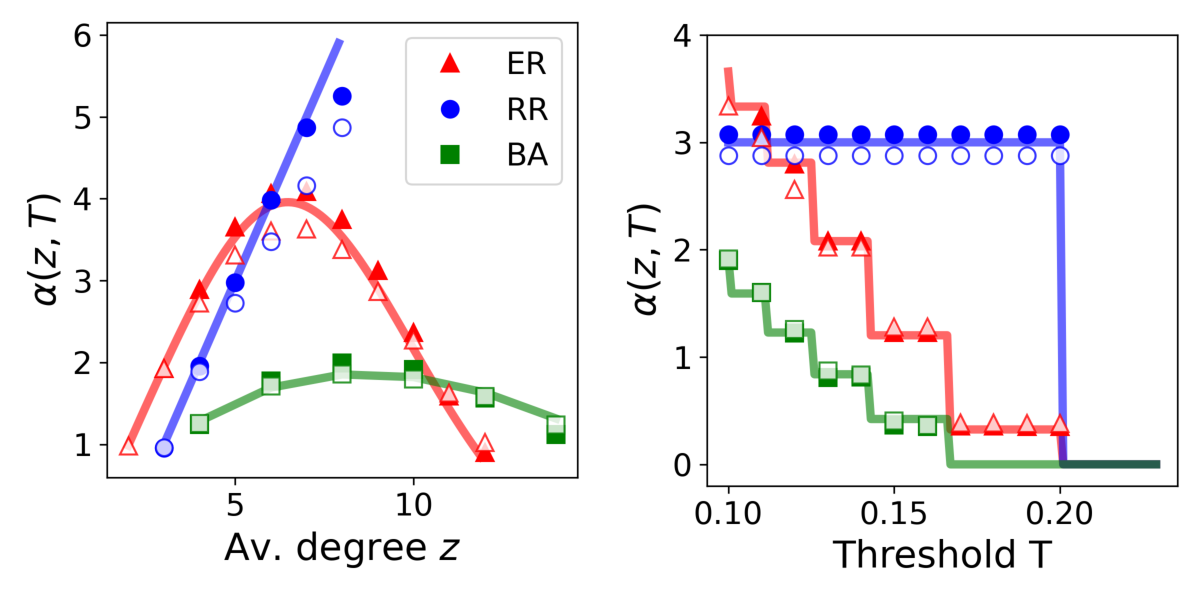
\includegraphics[width=0.7\columnwidth]{Figs/Aging_Threshold/ENDO.pdf}
    \caption[Exponent for the Granovetter-Watts model]{\label{fig:endo_exp} Exponent $\alpha$ for the original Granovetter-Watts model (empty markers) and $\delta$ for the version with endogenous aging (filled markers) for different values of the average degree $z$ (and $T = 0.1$) \textbf{(left)} and as a function of $T$ for fixed $z$ \textbf{(right)}. Different markers indicate results from Monte Carlo simulations with different topologies: red triangles indicate an Erd\H{o}s-R\'enyi (ER) graph, blue circles indicate a random regular (RR) graph and green squares indicate a Barab\'asi-Albert (BA) graph. In the right panel, the average degree is fixed $z = 5$ for ER and RR, and $z = 8$ for the BA. Predicted values by Eq. \eqref{eq:alpha} (solid lines) fit the results for each topology. System size is fixed at $N = 4 \times 10^6$ for the original model and $N = 3.2 \times 10^5$ for the version with aging.}
\end{figure}

As an ansatz, we assume that timing interactions can be effectively decoupled from the adoption process so the solution of Eq. \eqref{eq:AME_Threshold} can be written as
\begin{equation}
    \label{eq:assumption1}
    x^{+}_{k,m,j}(t) = x^{+}_{k,m}(t) \, G_{j} (t),
\end{equation}
where $x^{+}_{k,m}$ is the fraction of non-adopters with degree $k$ and $m$ infected neighbors $x^{+}_{k,m} = \sum_{j} x^{+}_{k,m,j}$ and there is an age distribution $G_{j} (t)$, independent of the adoption process.

If we sum over the variable age $j$ in Eq. \eqref{eq:AME_Threshold}, we can rewrite the following rate equations for the variables $x^{+}_{k,m}$
\begin{equation}
    \label{eq:threshold_AME_red}
    \frac{d x^{+}_{k,m}}{dt}  = \,  - \langle p_A \rangle \, \theta(m - kT)\, x^{+}_{k,m} - (k - m) \, \beta^s \,  x^{+}_{k,m} + (k - m + 1)\, \beta^s \,  x^{+}_{k,m-1},
\end{equation}
where aging effects are  just included in $\langle p_A \rangle(t)$: 
\begin{equation}
    \langle p_A \rangle(t) = \sum_{j = 0}^{\infty} p_A(j) \, G_j (t).
\end{equation}

Using the definition of the fraction of $k$-degree adopters $x^{-}_{k} (t)$,
\begin{equation}
    x^{-}_{k}(t) = 1 - \sum_{j=0}^{\infty} \sum_{m = 0}^k x^{+}_{k,m,j},
\end{equation}

and along the lines of Ref.~\cite{gleeson-2013}, we use the following ansatz

\begin{equation}
    x^{+}_{k,m} = (1 - x^{-}_{k} (0)) \, B_{k,m}[\phi],
\end{equation}

\begin{figure}
    \centering \captionsetup{font=sf}
    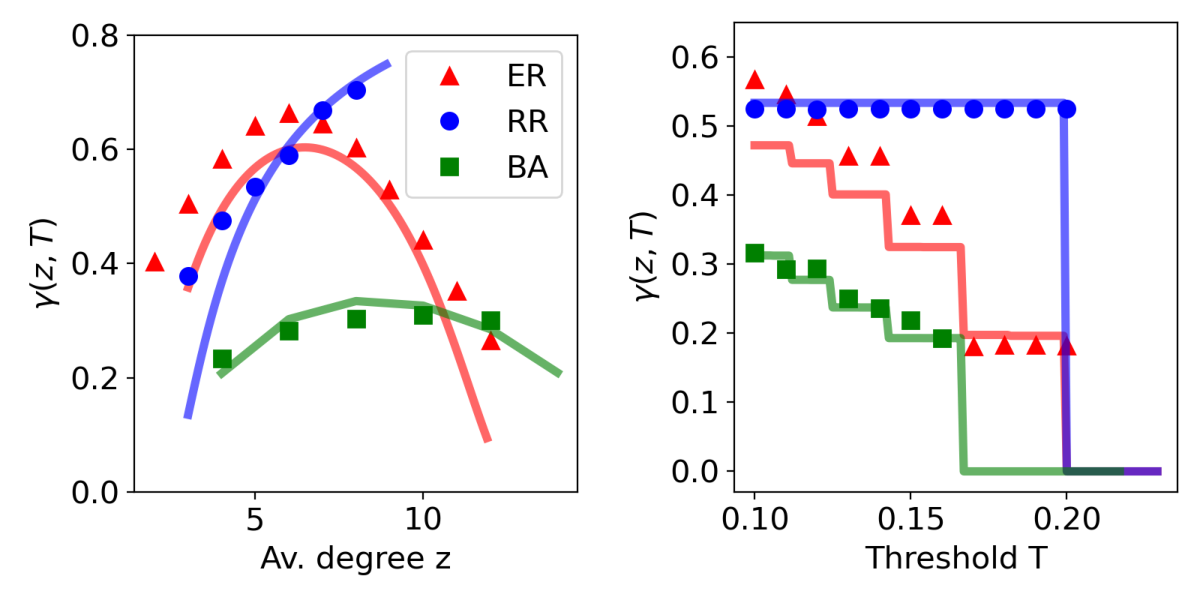
\includegraphics[width=0.7\columnwidth]{Figs/Aging_Threshold/EXO.pdf}
    \caption[Exponent $\gamma$ for the Granovetter-Watts model with exogenous aging]{\label{fig:exo_exp} Exponent $\gamma$ for the Granovetter-Watts model with exogenous aging for different values of the average degree $z$ ($T = 0.1$) \textbf{(left)} and as a function of  $T$ for fixed $z$ \textbf{(right)}. Different markers indicate results from Monte Carlo simulations with different topology: red triangles indicate an Erd\H{o}s-R\'enyi (ER) graph, blue circles indicate a random regular (RR) graph and green squares indicate a Barab\'asi-Albert (BA) graph. In the right panel, the average degree is fixed $z = 5$ for ER and RR, and $z = 8$ for the BA. Predicted values by numerical integration of Eqs. \eqref{eq:PA} (solid lines) fit approximately the results for each topology. System size is fixed at $N = 3.2 \times 10^5$.}
    \end{figure}

where $B_{k,m}[\phi]$ is the binomial distribution with $k$ attempts, $m$ successes and with success probability $\phi$. From this point, we derive from Eq. \eqref{eq:threshold_AME_red} a reduced system of two coupled differential equations for the fraction of adopters $x^{-}(t) = \sum_k p_k x^{-}_{k} (t)$ and an auxiliary variable $\phi (t)$ (see details in Ref.~\cite{gleeson-2013}):
\begin{equation}
    \label{eq:PA}
        \frac{d x^{-}}{dt} = \langle p_A \rangle [ h(\phi) - x^{-} ], \quad \quad \frac{d \phi}{dt} = \langle p_A \rangle [ g(\phi) - \phi ],
\end{equation}
where $\phi(t)$ can be understood as the probability that a randomly chosen neighbor of a non-adopter node is an adopter at time $t$. The functions $h(\phi)$ and $g(\phi)$ are nonlinear functions of this variable $\phi$
\begin{align}
    h (\phi)  = & \,  \sum_{k=0}^{\infty} p_k\,  \left( x^{-}_{k} (0) + (1 - x^{-}_{k} (0))\,  \sum_{m = kT}^{k} B_{k,m}[\phi]\right),\nonumber\\
    \\
    g (\phi)  = & \, \sum_{k=0}^{\infty} \frac{k}{z}\,  p_k \,  \left( x^{-}_{k} (0) + (1 - x^{-}_{k} (0)) \, \sum_{m = kT}^{k} B_{k-1,m}[\phi]\right). \nonumber
\end{align}
 When $\langle p_A \rangle$ is replaced by a constant, Eqs. \eqref{eq:PA} reduce to previous results for the original model~\cite{gleeson-2008}.
 
Determining the distribution $G_j (t)$ a priori is not easy. For endogenous aging, all non-adopters have the same age at each time step and $G_j (t) = \delta(j-t)$ (where $\delta(\cdot)$ is the Dirac delta function). Therefore, $\langle p_A \rangle = 1/(t+2)$. The numerical solution of Eq. \eqref{eq:PA} gives a good agreement with Monte Carlo simulations (see Fig. \ref{fig:exo_endo_evo}(a-c)). For the case of exogenous aging, the reset of the internal clock makes more difficult a choice for $G_j (t)$.  Inspired on the stretched exponential behavior of $x^{-}(t)$ observed from Monte Carlo simulations, we propose $\langle p_A \rangle = 1/(t+2)^\mu$. For $\mu = 0.75$, the numerical solutions of Eq. \eqref{eq:PA} gives a very good agreement with our Monte Carlo simulations (see Fig. \ref{fig:exo_endo_evo} (d-f)).

\subsection{\label{subsec Analytical results} Analytical results}


To obtain an analytical result for the cascade condition and for the exponents of the predicted exponential, stretched-exponential and power law cascade dynamics that we fitted from Monte Carlo simulations, we need to go a step beyond the numerical solution of our approximated differential equations (Eqs. \eqref{eq:AME_Threshold} and \eqref{eq:PA}). 
%Although the approximate master equation solutions give a good agreement with Monte Carlo simulations, are not able to confirm the cascade condition and the predicted exponential, stretched-exponential and power law cascade dynamics that we fitted from Monte Carlo simulations. We need further approximations to derive analytically the dynamics and the exponent dependence with the control parameters.

%To obtain the cascade condition, we follow the methodology from Ref.~\cite{gleeson-2007}. 
For a global cascade to occur, it is needed that the variable $\phi(t)$ grows with time. If we assume a small initial seed ($x^{-}_{k} (0) \; \to \; 0$), Eq. \eqref{eq:PA} can be rewritten as in Ref.~\cite{gleeson-2007}
\begin{equation}
    \label{eq:pre_lin}
    \frac{d \phi}{dt}  = \langle p_A \rangle \, \left( -\phi + \sum_{k=1}^{\infty} \frac{k}{z} \, p_k \, \sum_{m = k\, T}^{k} B_{k-1,m} [\phi] \right).
\end{equation}
Rewriting the sum term as $\sum_{l=0}^{\infty} C_l \, \phi^l$, with coefficients 
\begin{equation}
    \label{eq:coef_phi}
    C_l = \sum_{k=l}^{\infty} \sum_{m=0}^{l} { k-1 \choose l} \, {l \choose m} \, (-1)^{l+m} \, \frac{k}{z} \, p_k \, \theta\left(m/k - T \right),
\end{equation}
we linearize Eq. \eqref{eq:pre_lin} around $\phi = 0$:
\begin{equation}
    \label{eq:linear}
    \frac{d \phi}{dt} \approx  \langle p_A \rangle \, ( C_1 -1) \, \phi.
\end{equation}
The solution for Eq. \eqref{eq:linear} is then
\begin{equation}
    \label{eq:phi_general}
    \phi(t) = x^{-}_{0}\,  e^{(C_1 - 1) \, \int_0^t \langle p_A \rangle (s) \, ds},
\end{equation}
given that $ \phi(0) = x^{-}_{0}$.

Linearization is useful to determine the time dependence of the cascade process.  Assuming a small initial seed and rewriting the term $h(\phi)$ as  $ \sum_{l=0}^{\infty} K_l\,  \phi^l $, the linearized equation for the fraction of adopters $x^{-}(t)$ becomes
\begin{equation}
    \label{eq:linear_r}
    \frac{d x^{-}}{dt} \approx  \langle p_A \rangle\,  ( K_1 -1)\, \phi,
\end{equation}
where the coefficients $K_l$ are
\begin{equation}
    \label{eq:coef_rho}
    K_l = \sum_{k=l}^{\infty} \sum_{m=0}^{l} { k \choose l} \, {l \choose m} \, (-1)^{l+m}\,  p_k \, \theta\left( m/k - T \right).
\end{equation}

A solution for the fraction of adopters $x^{-}(t)$ can be obtained from  Eqs. \eqref{eq:phi_general} and \eqref{eq:linear_r}.  For the case of the Granovetter-Watts model without aging, setting $\langle p_A \rangle = 1$,  the solution is an exponential cascade dynamics
\begin{equation}
    x^{-}(t) = x^{-}_{0} \, e^{(C_1 - 1)\, t}.
\end{equation}
Therefore, the number of adopters $x^{-} (t)$ follows an exponential increase with exponent $\alpha(z,T)$:
\begin{equation}
    \label{eq:alpha}
    \alpha(z,T) = C_1 - 1 = \sum_{k=0}^{\lfloor 1/T \rfloor} \frac{k \, (k - 1)}{z}\, p_k - 1,
\end{equation}
where $C_1$ is computed from Eq. \eqref{eq:coef_phi}. 

For endogenous aging, the same derivation is valid to determine the exponents $\delta(z,T)$. Using $\langle p_A \rangle = 1/(t+2)$, the fraction of adopters follows a power law dependence,
\begin{equation}
    \label{rho_endo}
    x^{-}(t) = x^{-}_{0} \, \left( \frac{t+2}{2} \right)^{(C_1 - 1)}.
\end{equation}
The exponent reported for the power law cascade dynamics $\delta(z,T)$ turns out to be, therefore, the same exponent as the one for the exponential behavior where there is no aging:  $\delta(z,T)= \alpha(z,T)= C_{1} - 1$. Fig. \ref{fig:endo_exp} compares the prediction of Eq. \eqref{eq:alpha} with the results computed from Monte Carlo simulations. There is a good agreement for both Barab\'asi-Albert and Erd\H{o}s-R\'enyi networks for all values of $T$ and $z$. For a random-regular graph, the predicted dependence, $\alpha(z) = z - 2$, is not a good approximation for large $z$. This is because the presence of small cycles increases importantly in a random-regular graph as the average degree $z$ grows~\cite{wormald_1999} and the locally-tree assumption made for the derivation of the rate equations (Eq. \eqref{eq:AME_Threshold}) is not valid anymore. A different approach is necessary for clustered networks (as in Ref.\cite{Leah2022} for the Granovetter-Watts model). 

Moreover, from Eq. \eqref{eq:linear}, we can extract the cascade condition for the Granovetter-Watts model in general. Since $\langle p_A \rangle(t)$ is always positive, global cascades occur when $(C_1 - 1) > 0 $, so the cascade condition is:
\begin{equation}
    \label{eq:umbral}
    \sum_{k=0}^{\lfloor 1/T_c \rfloor} \frac{k \, (k - 1)}{z}\, p_k = 1
\end{equation}
This cascade condition does not depend on the aging term $\langle p_A \rangle(t)$ and thus, it is the same as for the Granovetter-Watts model without aging. In Fig. \ref{fig:umbral}, the red solid line is the result of this analytical calculation, and it is in good agreement with the numerical results. 

\begin{figure}
    \centering \captionsetup{font=sf}
    \includegraphics[width=0.5\columnwidth]{Figs/Aging_Threshold/LATT_PLOT.png}
    \caption[Cascade spreading of the Granovetter-Watts model in a lattice]{\label{fig:evo_lat} Cascade spreading of the original Granovetter-Watts model \textbf{(a)} and the versions with endogenous (reset if adopts) \textbf{(b)} and exogenous (reset if activates) \textbf{(c)} aging on a Moore neighborhood lattice with size $N = L \times L$, $L = 405$. Yellow and purple nodes are adopters and non-adopters, respectively. Time increases from left to right. Initial seeds are selected favoring cascades: one agent and all him/her neighbors are set as adopters at the center of the system.}
\end{figure}

For exogenous aging, an analytical expression for the exponent $\gamma(z,T)$ is not obtained following this methodology. Still, we can fit the exponent from the numerical solutions in Fig. \ref{fig:exo_endo_evo} (d-f). Fig.\ref{fig:exo_exp} shows a good comparison between the exponent calculated from the numerical solutions and the one calculated from  Monte Carlo simulations. The dependence of $\gamma(z,T)$ with the parameters $z$ and $T$ is qualitatively similar to the dependence of  $\alpha(z,T)$.

\section{\label{sec:Lattice} Results on a Moore lattice}

The Granovetter-Watts model in a two-dimensional regular lattice with a Moore neighborhood (nearest and next nearest neighbors) has a critical threshold (cascade condition) $T_c = 3/8$~\cite{centola-2007}. Below this value, cascade dynamics follows a power law increase in the density of adopters $x^{-}(t)$, which does not depend on the threshold value $T$~\cite{centola-2007}. In Fig. \ref{fig:evo_lat}a, we show a typical realization of this model: From an initial seed, the adoption radius increases linearly with time until all agents adopt the technology.

When aging is considered, cascade dynamics become much slower and a dependence on $T$ appears. When the aging mechanism is exogenous, Monte Carlo simulations indicate cascade dynamics following a power law $x^{-}(t) \approx t^{\zeta(T)}$. Qualitatively, we observe that while in the case without aging there was a soft interface between adopter and non-adopters, aging causes a strong roughening in the interface and the presence of non-adopters inside the bulk (see Fig. \ref{fig:evo_lat}c). In addition, the exponent values fitted from Monte Carlo simulations allow us to collapse curves for different system sizes (see Fig. \ref{fig:lattice}a). Due to finite size effects, the interface between adopters and non-adopters eventually reaches the borders of the system and the remaining non-adopters, in the bulk, will slowly adopt with the density of adopters following the functional shape $x^{-}(t) = 1- 1/(t+2)$.

Fig.\ref{fig:evo_lat}b shows the dynamics towards global adoption for endogenous aging. In comparison with the case of exogenous aging, we do not observe strong interface roughening between adopters and non-adopters, because non-adopters are not present in the bulk. Monte Carlo simulations indicate a very slow increase of the density of adopters $x^{-}$, similar to a power-logarithmic growth  $x^{-}(t) \approx (\log(t))^{\nu}$, with a threshold dependent exponent $\nu(T)$  (Fig. \ref{fig:lattice}b). Our general approximation used for complex networks assumes a tree-like network, and it is not appropriate for the Moore lattice. 

\begin{figure}
    \centering \captionsetup{font=sf}
    \includegraphics[width=\columnwidth]{Figs/Aging_Threshold/FIGA.pdf}
    \caption[Cascade dynamics snapshots in a lattice]{\label{fig:lattice} Cascade dynamics of the Granovetter-Watts model with exogenous \textbf{(a)} and endogenous \textbf{(b)} aging on a Moore neighborhood lattice. Different colors indicate different values of the threshold $T$. Different markers indicate the results of Monte Carlo simulations with different system size $N = L \times L$:  $L = 50$ (crosses), $100$ (triangles), $200$ (circles) and $400$ (squares). In (a), time is scaled according to size $\tau = L^{2 / \zeta}$. Discontinuous solid lines indicate a power law behavior with exponent $ \zeta = 4/3$ (blue), $1$ (red) and $2/3$ (green). In (b), the system sizes are not scaled due to the slow dynamics. Discontinuous solid lines indicate a power-logarithmic behavior, $x^{-}(t) \, N \sim \log(t)^{\nu} $, with exponent $ \nu = 7/3$ (blue), $2$ (red) and $5/3$ (green).}
\end{figure}
    

\section{\label{sec:Summary and Conclusions} Summary and discussion}

We have addressed in this chapter the role of aging in general models with binary-state agents interacting in a complex network. Temporal activity patterns are incorporated by means of a variable that represents the internal time of each agent. We have developed an approximate Master Equation for this general situation. In this framework, we have explicitly studied the effect of aging in the Granovetter-Watts model as a paradigmatic example of Complex Contagion processes. Aging implies a lower probability to change state when the internal time increases. We considered  two aging mechanisms: endogenous aging, in which the internal time measures the persistence time in the current state, and exogenous aging, in which the internal time measures the time since the last update attempt.

%To summarize, we have explored the effect of exogenous and endogenous aging in a stochastic binary-state model. Autonomous agents have now an internal time counting the persistence time in the same state (or since a reset for the exogenous aging mechanism). We use Threshold model as a paradigmatic example where, even for the original model, one needs to go beyond heterogeneous mean field to have agreement with Monte Carlo simulations.

Our theoretical framework with some approximations to attain analytical results provide a good description of the results from Monte Carlo simulations for Erd\H{o}s-R\'enyi, random-regular and Barab\'asi-Albert networks. For these three types of complex networks, we found that the cascade condition $T_c$ (critical value of the threshold parameter $T$ as a function of mean degree $z$ of the network) for the full spreading from an initial seed is not changed by the aging mechanisms. However, aging modifies in non-trivial ways cascade dynamics of the process. The exponential growth with exponent $\alpha(z,T)$ of the density of adopters in the absence of aging becomes a power law with exponent $\delta(z,T)$ for endogenous aging, and a stretched exponential characterized by an exponent $\gamma(z,T)$ for exogenous aging. We have analyzed the exponents' dependence with the order parameters $\alpha(z,T)$, $\delta(z,T)$, $\gamma(z,T)$ and shown that $\delta(z,T)=\alpha(z,T)$, for which an analytical expression is obtained.

Our general theoretical framework, based on the assumption of a tree-like network, is not appropriate for a regular lattice. In this case, we have been only able to run Monte Carlo simulations. Our results indicate that  exogenous aging gives rise to adoption dynamics characterized by an increase in the interface roughness, by the presence of non-adopters in the bulk, and by a power law growth of  the density of adopters with exponent $\zeta (T)$, while in the absence of aging $\zeta = 2$ independently of $T$. Endogenous aging, on the other hand, produces very slow (logarithmic-like) dynamics, with a threshold-dependent exponent $\nu(T)$.

%In addition, the case of lattice is studied in a separate scheme. When aging is 

%We build an approximate master equation, general for any binary-state model with temporal activity patters. The numerical resolution of the AME shows a very good agreement with Monte Carlo simulations (see Fig.\ref{fig:models}). In particular, for the case of Threshold model with aging, the AME is reduced to a system of only two differential equations when we decouple the age distribution from the adoption process. It is shown that numerical integration also presents a good agreement with Monte Carlo simulations.

%To predict the exponential (from the original model) and power law behavior (endogenous aging), we linearize the previous system of differential equations. An analytical expression for the exponents is extracted, general for any threshold $T$ and any network (with $p_k$) with average degree $z$ (see Eq.\eqref{eq:alpha}). Exponents from the exogenous aging dynamics are compared with the numerical integration solution of the reduced system of differential equations (Eq. \eqref{eq:PA}).

%Since we focused only on infinite, uncorrelated networks with negligible clustering, we observe that the approximation is not valid for random-regular graphs with high degree. Therefore, a generalization of the AME to networks with high clustering and degree-degree correlations is needed. Moreover, would be interesting a different approach with a pair approximation, including the adoption dependence also to the age distribution. Another approach to binary-state dynamics with timing interactions is consider the stochastic and size effects into the derivation (as in Ref.\cite{peralta-2020B}).

%In addition, the case of lattice is studied in a separate scheme. When aging is included, a dependence on the threshold parameter of the model $T$ appears naturally. For the exogenous aging, dynamics change to a power law behavior , with an exponent that depends on $T$, universal for any system size. This aging mechanism also show particular behavior as interface branching and presence of non-adopters inside the adoption bulk. On the other hand, the endogenous aging shows a very slow adoption increase similar to logarithmic. For large system sizes, to reach the fully-adopted state takes a large number of time steps. Since the dependence on parameter $T$ has a particular shape for both cases, further work would include taking the continuous limit to obtain an analytical derivation of the exponent to compare with Monte Carlo simulations. 

This study highlights the importance of non-Markovian dynamics in general  binary-state dynamics and, specifically, in the Granovetter-Watts model. For the problem of innovation adoption that this model addresses, we show how persistence times have an important impact on the adoption cascade. Further work in this direction would be to categorize technologies according to the adoption curve, to show if the system has important resistance to the previous technology (endogenous aging) or a balance between memory and external influence or advertisement (exogenous aging). Furthermore, the theoretical framework presented here gives a basis for further investigations of the memory effects and non-Markovian dynamics in networks, and in particular for  binary-state models with aging. Still, a number of theoretical developments remain open for future work, such as the consideration of stochastic finite size effects~\cite{peralta-2020B}, or extending this framework to tri-state models. Also, proper approximations need to be developed to account for some of our numerical results for random-regular networks with high degree, as well as for high clustering, degree-degree correlations networks and for regular lattices, including continuous field equations for this latter case. 
